\section{Ionized Gas}
A plasma is considered to be a form or subset of ionized gas. That is, a
volume of neutral atoms or molecules, of which some fraction has been
separated into electrons and ions. For a sufficiently large number of
particles, the behavior of each species in the ionized gas can be
described by a continuous distribution function which specifies the
number of particles with a specific range of velocities, in a specific
volume, at a specific time. This function is denoted
$f_\alpha(\vec{r_\alpha}, \vec{v_\alpha}, t)$, where the subscript
$\alpha$ denotes the species, $f$ is the probability distribution,
$\vec{r}$ is the position, $\vec{v}$ is the velocity, and $t$ is the
time.

The behavior of $f_\alpha$ can be shown to be governed by the Boltzmann
equation,
\begin{equation}\label{eq:boltzmann}
  \frac{\partial f_\alpha}{\partial t} + \vec{v_\alpha}\cdot\nabla f_\alpha +
  q_\alpha \left(\vec{E} + \vec{v_\alpha}\times\vec{B}\right)
  \cdot \nabla_v f_\alpha = \left( \frac{\partial f_\alpha}
  {\partial t}\right)_\mathrm{coll}.
\end{equation}
Here, $q$ is the charge of the species, $\vec{E}$ is the electric field,
$\vec{B}$ is the magnetic field, and $\partial f_\alpha/(\partial
t)_\mathrm{coll}$ is a term which represents changes to the distribution
function as a result of collisions. Coupled with Maxwell's equations,
equation~\ref{eq:boltzmann} provides a complete description of the
behavior of the fields and particles in a plasma.

For a species in equilibrium in the absence of external forces
(($\partial f_\alpha/\partial t)_\mathrm{coll} = 0$) it can be shown
that
\begin{equation}\label{eq:mb}
  f_\alpha(v_\alpha) =
    n_\alpha\left( \frac{m_\alpha}{2\pi \kB T_\alpha}\right)^{3/2}
   \exp\left(-\frac{m_\alpha v_\alpha^2}{2\kB T_\alpha}\right),
\end{equation}
where $n$ is the total density of the species, $m$ is the particle mass,
$\kB$ is Boltzmann's constant, and $T_\alpha$ is the temperature of the
species. It must be emphasized that this solution only applies to
situations where the species can be considered to be in equilibrium.
Strong gradients and large electromagnetic fields can both drive a
distribution far from its equilibrium condition. This is particularly
important when plasmas are discussed in the context of temperature.

Solutions of the equation~\ref{eq:boltzmann} in anything but this simple
case can be very challenging. It most situations, it is reduced to more
tenable equations by integrating over the velocity-space (leaving $f$ as
only a function of space and time). The first so-called moment is often
called the conservation equation or continuity equation,
\begin{equation}\label{eq:cont}
  \frac{\partial n_\alpha}{\partial t} + \nabla \cdot (n_\alpha \vec{u_\alpha})
  = G_\alpha - L_\alpha.
\end{equation}
In this case, $\vec{v}$ has been replaced by a mean velocity $\vec{u}$.
We have also introduced terms losses ($L$) and gains ($G$) in the
species density.

The definition of the mean velocity can be obtained by multiplying
equation~\ref{eq:boltzmann} by $v$ and integrating over velocity-space.
This is referred to as the second moment. The result is an equation
expressing the conservation of momentum for the species. The actual
equation will not be reproduced here, but it forms the basis for the
two-fluid approximation of a plasma. In the course of developing the
second moment an additional term, the pressure tensor, is introduced
which can only be defined by the third moment of
equation~\ref{eq:boltzmann}. In fact, each additional moment introduces
a new term, \emph{ad infinitum}. For most cases, the first two or three
moments suffice, after the sequence is terminated by the use of an
additional assumption.

For our purposes, one more moment will suffice. Multiplying by $mv^2/2$,
integrating over velocity-space, and assuming that the pressure is
isotropic, produces the energy conservation equation,
\begin{equation}
  \frac{\partial}{\partial t}\left(\frac{3}{2}p_\alpha\right) 
  + \nabla\cdot\frac{3}{2} (p_\alpha\vec{u}_\alpha)
  + p_\alpha\nabla\cdot\vec{u}_\alpha
  + \nabla\cdot\vec{q}_\alpha
  = \frac{\partial}{\partial
  t}\left(\frac{3}{2}p_\alpha\right)\bigg|_\mathrm{coll}.
\end{equation}
In this case, $p$ represents the plasma pressure, and $\vec{q}$ is the
heat flow. The first term on the \textsc{lhs} represents the total
energy contained by the species, the second term is the energy flux in
and out of the volume, and the third term accounts for changes due to
compression or expansion. The \textsc{rhs} is the collision operator
which describes energy added or removed from the system as a result of
collisions.

\section{Plasma Criteria}
While equations above can equally describe an ionized gas or a plasma,
the two are conceptually distinct. A plasma is unique in that its
dynamics are governed by long range electromagnetic forces, unlike gases
in which short-range collisions dominate. As a result, plasmas
frequently feature large scale structure and organization. Examples of
these structures are ubiquitous in astronomy where phenomena such as the
aurora borealis, coronal mass ejections, and even interstellar media all
qualify as forms of plasma. How then, does one define a plasma? There
are three criteria required of an ionized gas in order for it to be
considered a plasma.

\subsection{$\lambda_D < L$}
An ionized gas is composed of both positive and negative charges,
usually some combination of ions and electrons. If an electrical
perturbation is introduced, the charge particles will tend to rearrange
themselves to shield out the effect of the perturbation. A plasma is an
ionized gas which is sufficiently large for this shielding effect to
occur. The length scale of this shielding effect is referred to as the
Debye length, denoted $\lambda_D$. The Debye length can be shown to be
equal to $\sqrt{\epsilon_0T_e/(en_0)}$, where $\epsilon_0$ is the vacuum
permittivity, $T_e$ is the electron temperature, and $n_0$ is the plasma
density. If the characteristic length scale of the ionized gas is $L$,
then $\lambda_D < L$ for it to be considered a plasma.

\subsection{$n_0(4\pi \lambda_D^3/3) >> 1$}
However, the previous condition is necessary, but not sufficient for
shielding to occur. It is possible to have an ionized gas in which the
Debye length is smaller than the characteristic length scale, but in
which there are too few charged particles for shielding to occur. More
simply put, it would be impossible for a single electron to shield out
even the smallest of perturbations. For that reason, the number of
particles in a Debye sphere must be greater than unity in a plasma.

\subsection{$\omega_p > \nu$}
If an ionized gas meets the two aforementioned conditions, it may still
not exhibit the large scale structure of plasma if the collision
frequency with neutral particles is too high. In this case, the behavior
of the ionized gas would be determined more by the random collisions
with gas particles than the long-range electromagnetic forces. As a
result, the characteristic oscillation frequency of a plasma (or plasma
frequency) $\omega_p$ must be greater than the neutral collision
frequency, $\nu$. Here, $\omega_p = \sqrt{e^2n_0/(\epsilon_0
m_e)}$.

In spite of this range of requirements, there are a large number of
natural and man-made plasmas. Figure~\ref{fig:regimes}
\begin{figure}
  \centering
  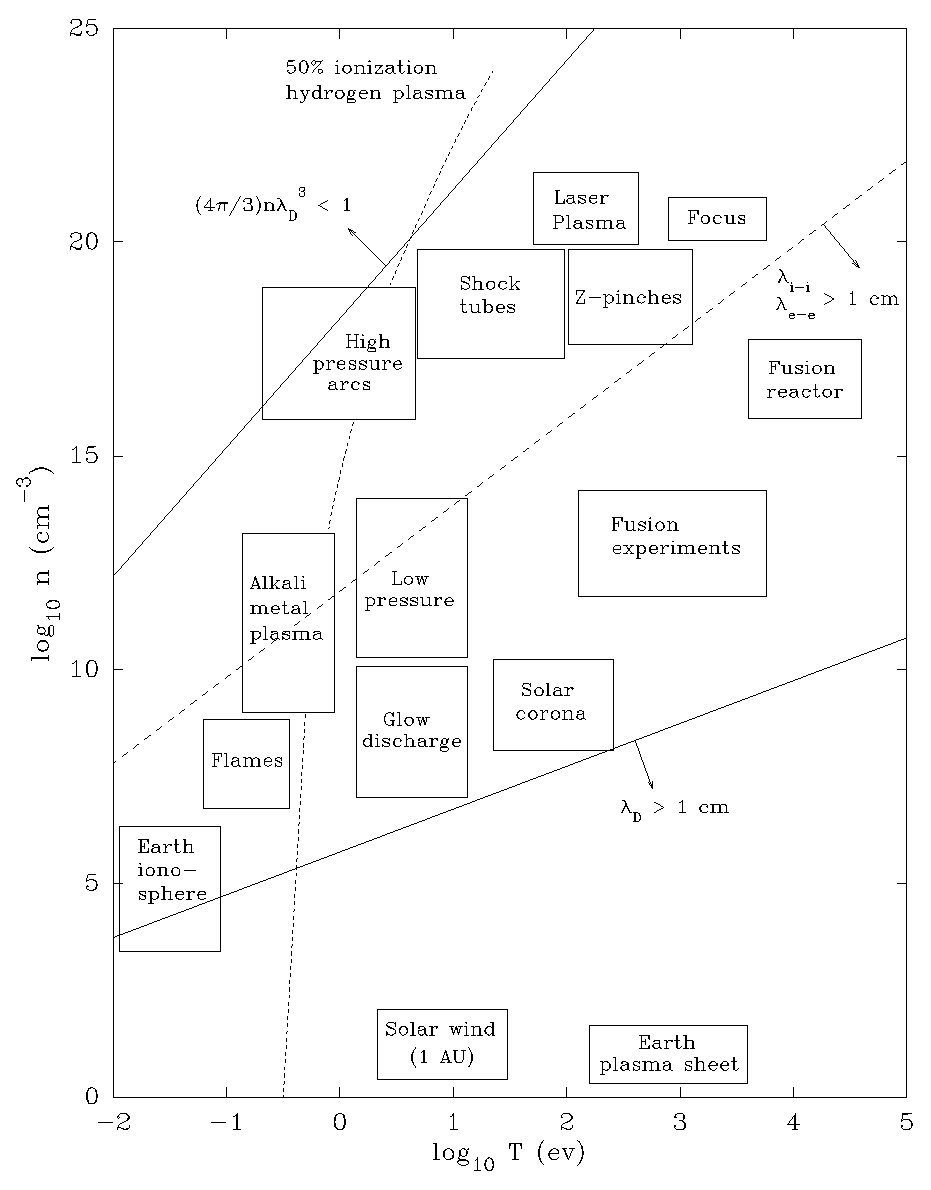
\includegraphics{./chapters/theory/figures/regimes.eps}
  \caption{Illustration of the various regimes of plasma in terms of
electron temperature and density \cite{Huba2011}.}
  \label{fig:regimes}
\end{figure}
shows several categories of plasma, plotted as a function of their
electron density and temperature. As can be seen, the electron densities
span seven decades, and the densities cover in excess of 20.

\section{Streamer Discharge}
The Boltzmann equation is a continuous, statistical description of a
plasma. By comparison, the initial breakdown of a plasma is a
discontinuous process marked by its stochasticity. The initiation of a
discharge is the result of electron avalanches which may occur randomly
throughout the discharge, particularly without any form of
preionization. Often, the seed electrons for a plasma result from
ionizing cosmic rays which generate a few electrons per
cubic-centimeter. This has been verified with measurements of the
statistical lag in Townsend breakdown.

Briefly, the Townsend mechanism begins with some small number of primary
electrons between two electrodes. In the presence of a sufficient
electric field, the electron population exponentiates as they traverse
the anode-cathode gap. The collection of the electrons at the anode is
balanced out by the emission of secondary electrons from cathode as a
result of ion impact. The time required for an electron to drift across
the gap determines the formation time of a Townsend discharge, and the
secondary electron emission processes play an important role in
sustaining the discharge.

Conversely, the \acs{rpnd} is fundamentally similar to a streamer
discharge where secondary emission processes are unimportant, and space
charge plays an important role. Consider a single electron between two
electrodes, as seen in (a) of figure~\ref{fig:streamer}.
\begin{figure}
  \centering
  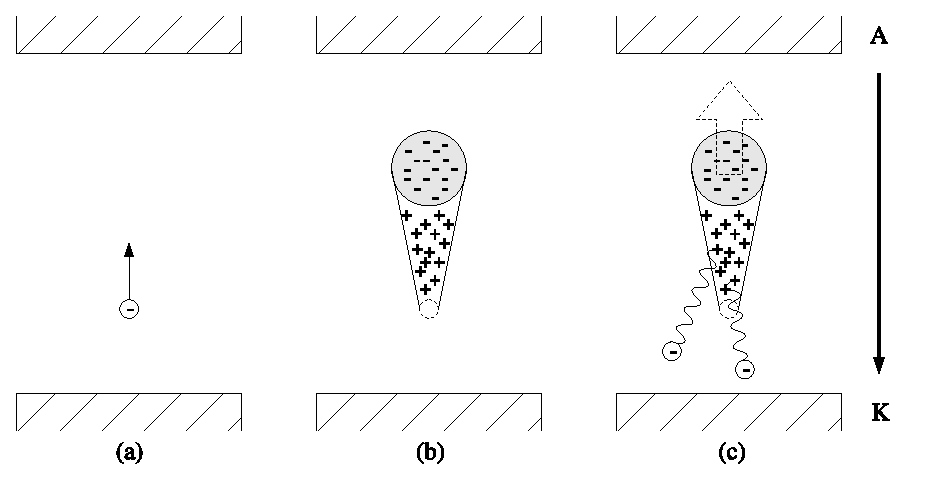
\includegraphics{./chapters/theory/figures/streamer.eps}
  \caption{An illustration of the development of a single streamer. (a)
    A seed electron is accelerated by the applied electric field. (b) The
    initial electron develops into an avalanche which leaves a large region
    of positive space charge, halting further advance. (c) The streamer
    propagates toward the cathode via photoionization and the anode via
    nonlocal electrons and photoionization.}
  \label{fig:streamer}
\end{figure}
The electron acquires energy from the applied electric field, and begins
to move in the direction of the anode. As the electron drifts, it
undergoes random collisions, some of which result in ionization. As long
as the charged particles do not significantly perturb the external
field, the new electrons also begin to drift resulting in an electron
avalanche.

On short time scales, the ions are essentially immobile as result of
their large mass. This produces a cone of positive space charge in the
wake of the electron avalanche, as seen in part (b) of
figure~\ref{fig:streamer}. The increasing radius of the avalanche with
distance occurs primarily as a result of collision-induced lateral
diffusion of the electrons. At some point, the space charge of the
positive ions becomes sufficient to shield the avalanche electrons from
the applied field. This halts the propagation of spherical region of
electrons in the streamer ``head.''

The length of this avalanche is equivalent to the minimum distance in
which a streamer can form. Following Levatter and Lin, the critical
avalanche distance can be expressed as
\begin{equation}
  \int_0^{\xi_c}\alpha(\xi')d\xi' = \ln\left(19.6 \epsilon_0 E \bar{\lambda_e}
                                           \bar{C_e}\xi_c/e\bar{u_e}\right),
\end{equation}
where $\xi_c$ is the critical avalanche length, $\xi$ is the overall
avalanche length, $\alpha$ is the first Townsend coefficient expressing
the number of electrons generated for a given distance and field, $E$ is
the applied field, $\bar{\lambda_e}$ is the electron mean free path,
$\bar{C_e}$ is the mean thermal velocity of the electron, and $\bar{u_e}
= \mu\dot{E}[t_0+\delta t/2]$ is the mean drift velocity of the
electron.


This can be expressed as a mobility, $\mu = u/E$, where $u$ is the drift
velocity and $E$ is the applied field. The mobility can be found by
empirical methods, or through solutions of the Boltzmann equation. Here,
we use approximate solutions of the Boltzmann equation found with the
program \smaller{BOLSIG+} \cite{Hagelaar2005} using the electronic cross
sections of Phelps \cite{Phelps2002}.

The distance it takes to form this critical level of space charge is the
minimum distance in which a streamer can form.

TODO: Develop Critical radius of streamer head

TODO: Develop size condition for streamer formation

At this point, several processes become important for the streamer to
continue its progress across the gap, displayed in part (c) of
giure~\ref{fig:streamer}. The large internal field of the streamer can
``inject'' electrons in the direction of the anode \cite{Kunhardt1980}.
In addition, excited atoms in the wake of the avalanche can emit
photons, ionizing the gas between the streamer head and the anode. These
electrons are subject to the large electric field between the anode and
streamer head, resulting in additional avalanches. Likewise,
photoionization can occur in the region between the tail of the streamer
and the cathode. The any photoelectrons generated in this region are
accelerated toward the tail of the streamer, resulting in additional
avalanches.

However, in the \acs{rpnd} these later processes in part (c) are not
critical to the formation of the volume discharge. Instead, as described
by Levatter and Lin \cite{Levatter1980}, a sufficiently large amount of
preionization results in a similarly large number of avalanches.
Provided these avalanches are close enough, the streamer heads will
overlap before reaching the critical electric field strength. This
action smooths out the strong local gradients that cause streamers to
filament and constrict.

TODO: HOMOGENEOUS DISCHARGE CONDITION

\section{Atomic Spectroscopy \& Notation}

Unlike physical probes, optical diagnostics are noninvasive and offer an
attractive approach to the measurement of plasma parameters. Careful
measurements of the light emitted from excited atomic states can yield electron
densities and temperatures, excited state densities and temperatures, electric
fields, and magnetic fields. The topic of spectroscopy is extensive and it is
neither necessary nor desirable to cover it in full. Instead we will only
consider what is necessary to understand the emissions from a singly-excited,
multi-electron atom.

An atom is composed of a small, positively charged nucleus, orbited by a
negatively charged electrons. The actual position of any single electron is
probabilistic and described by a wavefunction, as determined by solutions of the
Schr\"{o}dinger equation. Multiple possible wavefunctions or orbitals exist, and
the Pauli exclusion principle prevents more than one electron from possessing
the same orbital. Each orbital is identified by four quantum numbers,
\begin{itemize}
  \item $n=1,2,\ldots$: the principal quantum number,
  \item $l=0,1,\ldots,n-1$: the orbital angular momentum, and
  \item $s=\pm1/2$: the spin angular momentum.
\end{itemize}
The principal quantum number identifies the shell to which an electron belongs.
Each shell can contain a total of $2(2l+1)$ electrons, after which it is
considered full. Each shell has a series of subshells, defined by $l$ (using the
nomenclature $0,1,2,3,\ldots = s,p,d,f,\ldots$). 

The electrons of an atom possess potential energy as a result of their
separation from the nucleus. As $n$ and $l$ increase, so does the potential
energy, thus an electron in the 1s ($n=1$ and $l=0$) subshell has the lowest
possible potential energy. Each as a result of the exclusion principle, each
subshell can only contain up to $2(2l+1)$ electrons after which it is considered
full.

Absent from external influences, the subshells are populated with electrons so
as to minimize the potential energy of the system. This natural arrangement is
referred to as the ground state configuration. Often, but not always, the
subshells are filled sequentially and in order from lowest to highest $l$.
Provided some input energy, one or more of the electrons surrounding the atom
may transition to another orbital, increasing the potential energy of the
system. In low-temperature plasmas it usually one of the electrons from the
outermost or unfilled subshell to be excited.

In hydrogen-like atoms with a single electron in a single unfilled subshell, the
potential energy of any singly-excited configuration is uniquely determined by
this single outer electron. As a result, the initial and final states of the
atom can be uniquely identified based on the initial and final $n$ and $l$ of
aforementioned electron. In contrast, the potential energies of configurations
in noble gases and atoms with more than one electron in the valence shell are
determined by the collective effects of these outer electrons.

This necessitates an additional means of classifying the configuration of the
outer electrons. It turns out that the state of these types of atoms can be
specified based on their total orbital angular momentum $\bm{L}=\sum \bm{l}_i$,
the total spin, $\bm{S}=\sum \bm{s}_i$, and the total angular momentum,
$\bm{J}=\bm{L}+\bm{S}$, where $i$ are all the electrons of the unfilled shell.
In addition, each state can be said to have either even or odd parity, defined
as $(-1)^{\sum\bm{l}_i}$.

Together, these values can be used to express the term symbol for any particular
atomic state. For example, the so called triplet metastable state of helium can
be written as 1s2p$^3$P$^o_{0,1,2}$. This describes a helium atom with one
electron in the 1s subshell and a second atom in the 2p subshell. This
configuration has a total orbital angular moment of 1, odd parity (denoted by
the superscript `o'), a total spin of $1/2$ (the superscript $3$ is equal to
$2S+1$) and three possible values for the total angular momentum: 0, 1, or 2
which varies depending on the spin-orbit interaction.

These excited atomic states usually have finite lifetimes as the electrons in
the excited states will often transition to lower states. This can occur
spontaneously, through the emission of a photon, or via a superelastic collision
with another particle. In the case of spontaneous transitions, only certain ones
are allowed, as defined by a set of selection rules:
\begin{itemize}
  \item $\Delta S = 0$
  \item $\Delta L = \pm1$ or 0
  \item $\Delta J = \pm1$ or 0
  \item $L=0$ cannot transition to $L=0$
  \item $j=0$ cannot transition to $J=0$
\end{itemize}
These rules are determined using the electric dipole approximation. As a result,
some transitions forbidden by these rules can occur, though they occur with much
lower frequency.

Figure~\ref{fig:grotrian}
\begin{figure}
  \centering
  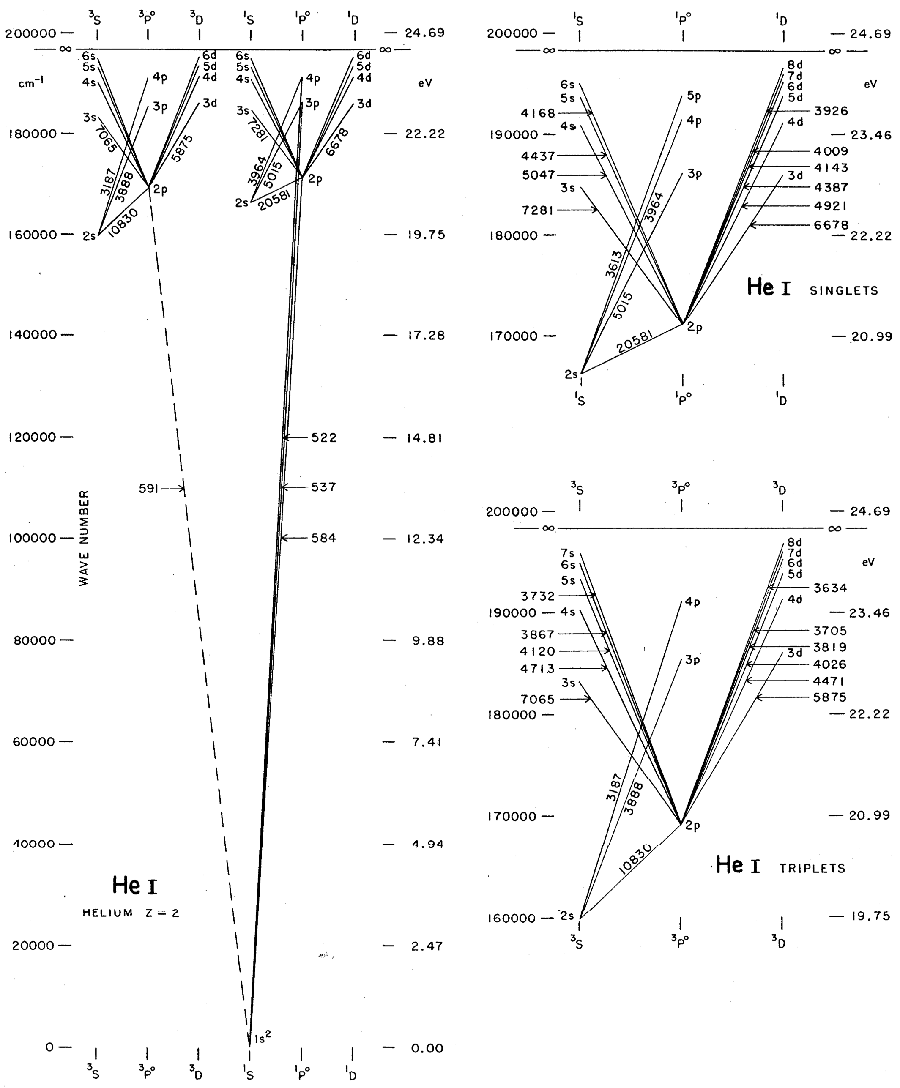
\includegraphics{./chapters/theory/figures/grotrian.pdf}
  \caption{A partial Grotrian diagram of neutral helium \cite{Moore1968}.}
  \label{fig:grotrian}
\end{figure}
is a diagram of the energy levels in neutral helium and the allowed transitions.
In this case, the atomic states are separated into the singlet and triplet
manifolds. The singlet manifold represents excited states where the electron
spins are anti-parallel, and the triplet manifold represents excited states
where the electron spins are parallel. As indicated by the first selection rule,
transitions between these two manifolds is forbidden, thus each is something of
a self-contained system.

\subsection{Spectral Lineshapes}

It is the transitions between these various excited states which concern
spectroscopy. Electrons which transition to lower energy states emit photons
which can be detected. Conversely, if an atom is subject to a photon with an
energy matching a transition, the photon may be absorbed. Both processes are
useful in determining the prevalence and dynamics of the excited states. This,
in turn, can be used to infer various plasma properties.

The light 

It is tempting to think that the energy spacing can be calculated exactly,
however there is always some variance about a central energy. This is called the
spectral lineshape, and it effects both the energy of the emitted photon in
radiative transitions, and the photons that an atom can absorb. Though these
variations can be attributed to quantum mechanical effects, the actual result
can derived from the so-called dipole approximation.

In this case, we envision a single electron oscillating about a large, heavy,
positive charge. The full details of this derivation are covered in Siegman
\cite{Siegman1986}, however we'll address some of the most pertinent portions
here. The response of a collection of atoms to an applied electric field can be
expressed as a quantity known as the susceptibility. This is generally defined
as
\begin{equation}
    \tilde{\chi}(\omega) \equiv
    \frac{\tilde{P}(\omega)}{\epsilon_0\tilde{E}(\omega)}
\end{equation}
where $\tilde{\chi}$ is the electric susceptibility, $\tilde{P}$ is the
macroscopic polarization, $\tilde{E}$ is the applied electric field, and
$\omega$ is the frequency of the applied field.

\paragraph{Natural Linewidth}
The electric susceptibility often possesses both a real and imaginary component.
Physically, these respectively represent the reactive and absorptive component
of the medium. Accounting for level-dependent effects, the standard
susceptibility for an atomic transition can be written as
\begin{equation}
    \tilde{\chi}_\mathrm{at}(\omega) = -j\frac{3}{4\pi^2}\frac{\Delta
    N\lambda^3\gamma_\mathrm{rad}}{\Delta\omega_a}\frac{1}{1
    + 2j(\omega - \omega_a)/\Delta\omega}
\end{equation}
where $\Delta N$ represents the population difference between the upper and
lower levels of the oscillator, $\lambda$ is the transition wavelength,
$\gamma_\mathrm{rad}$ is the natural radiative lifetime of the oscillator,
$\Delta\omega_a$ is the linewidth of the transition (for an unperturbed
atom, this is simply $\gamma_\mathrm{rad}$), and $\omega_a$ is the
angular frequency of the transition or oscillator.

This equation is generally known as the complex lorentzian. Separated into its
components it expresses both the absorptive and reactive properties of the
atomic medium. It also clearly susceptible to fields that are displaced from
$\omega_a$. This is the finite linewidth associated with atomic
emissions and absorption.

This linewidth affects each atom within the medium. Each atom will emit or
absorb radiation with a probability described by this susceptibility.
Consequently, this natural linewidth falls under the homogeneous category of
line broadening.

\paragraph{Pressure Broadening}
Also included in this category is pressure broadening, or more fundamentally,
dephasing. 

\subsection{Radiation Trapping}

\section{Collision Processes}
